
\section{Redundancy-based Cache Oblivious Data Layout Algorithm}

\subsection{Definitions}

Let us assume that the walkthrough scene data, including all the levels of details of the model, are partitioned into equal sized data blocks (say 4KB) called data units. This is the atomic unit of data that is accessed and fetched from the disk. Typically, vertices and triangles that are spatially together (and belong to the same level of detail), have high chances of being rendered together, and hence can be grouped together in a data unit. All the data units required to render a scene from a viewpoint is labeled as an {\em access requirement}. In order to minimize the number of access requirements, the navigation space in the walkthrough scene, which defines the space of all possible view points, is partitioned into grids and all the viewpoints within each grid is grouped together to define one access requirement. Thus the number of grid partitions define the number of access requirements. Clearly, primitives in a data unit can be visible from many viewpoints, and hence that data unit will be part of many access requirements. \\
\\
That was one example of data units and their access requirements. In general, the access requirements are determined by the application and are meant to be sets of data units that are likely to be accessed together. Given a linear ordering of data units that may eventually be the order in which they are stored in the hard drive, for an access requirement $A$, the total span of $A$ is the total number of data units between the first and last data units that use $A$. If a data unit is not required by $A$ but lies between the first and last unit of $A$ then it is still counted in the span of $A$. Figure \ref{singleAR} shows a set of data units and explicitly labels the blue access requirement in this set. The total number of data units between the first and last blue unit is 14 thus that is the total length of the blue access requirement.\\
\\
\begin{figure}[ht]
\centering
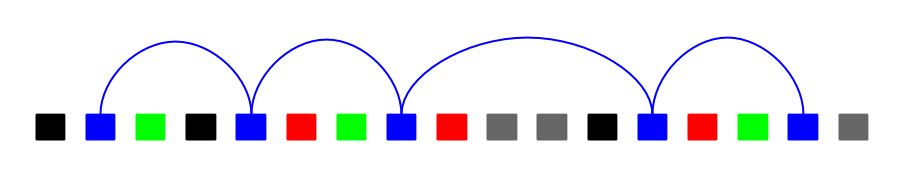
\includegraphics[width=3in]{SingleAR_start.png}
\caption{Illustration of linear order of data units and three example access requirements.
The lines connect data blocks that belong to the same access requirement
and represent parts of the span of an access requirement.}
\label{singleAR}
\end{figure}

\subsection{Seek Time Measure}
Given a linear order of data units and the access requirements, and assuming that each access requirement
is equally likely to be used, we would like to estimate the seek time for that application.
For each access requirement the read head of the hard disk has to move from the first data block to the last
irrespective of whether the intermediate blocks are read or skipped. Hence the span of an access requirement
is a measure of seek time - time taken to seek the last data unit starting from the first data unit.
Let $I$ be the set of access requirements and $A_i$ represent the span of the access requirement $i$.
Then estimated total seek time EST is given by 
\[
EST = \sum_{i \in I}{A_i}
\]
It is interesting to note that \cite{cacheobliviouslayout}
used span to measure the expected number of cache misses.
Typically, with every cache miss, the missing data will be sought in the disk and fetched,
thus adding to the seek time. Hence using span to measure the seek time is justified.


\subsection{Algorithm Overview}

In \cite{cacheobliviouslayout}, the only allowed operation on the data units is
the move operation and the optimal solution is computed using only that
operation. For our purposes, we are allowed to copy data units, move them, and
delete them if they are not used. Using these operations, our goal is to minimize EST
while keeping the number of redundant copies as low as possible. After constructing a cache oblivious layout 
of the data set to get an initial ordering of data units, we copy one data unit to another location, and reassign 
one or more of the access requirements that uses the old copy of the data unit to the new copy, such that the EST is reduced. 
If all the access requirements that used the old copy, now use the new copy of the data unit, then the old copy is deleted. 
We repeat this copying and possible deletion of individual data units until our redundancy limit has been reached. \\
\\
{\bf Blocks to Copy:} Note that the span of an access requirement does not
change by moving an interior data unit to another interior location. Cost can
be reduced only by moving the blocks, i.e. data units, that are at the either ends of the access
requirement. This observation greatly reduces the search space of data units to
consider for copying. For the sake of simplicity of the algorithm, we operate
on only one data block at a time. \\
\\
{\bf Location to Copy:} Based on the above observation, given an access requirement, we can possibly move the beginning or the end data units of an access requirement to its interior. This will reduce its span, thus reducing the EST for the layout. However, if the new location of the data unit is in the span of other access requirements, it increases the span of those accesses by one unit. We thus want to find a location in the span of the access requirement under consideration but is in the span of the least number of other access requirements. Such a location is identified using a simple linear search through the span of the access requirement. Figure \ref{singleARafterCopyOtherAR} shows the data units in figure \ref{singleAR} before the copying and highlights the gray access requirement that will be affected. As can be observed in figure \ref{singleARafterCopyOtherAR} the gray access requirement has had its span increased by 1. Even though we reduced the total span by 2 with the blue access requirement, we also increased the total span by 1 with the gray access requirement, yielding a net benefit of 1 data unit. Among all the spots in the interior of the blue access requirement, the one chosen had the least number of overlapping access requirements at 1.\\

\begin{figure}[ht]
\centering
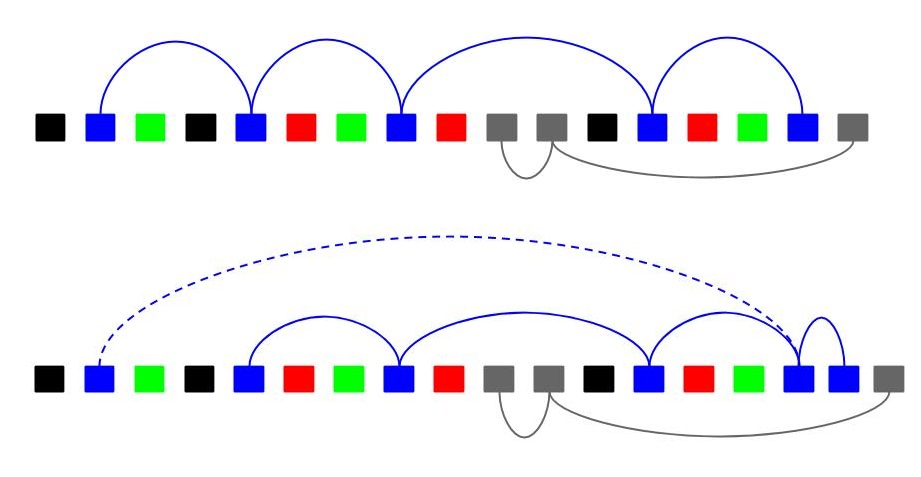
\includegraphics[width=3in]{SingleAR_afterCopy_otherARnoted.jpg}
\caption{The blue and gray access requirements before (top) and after (bottom) the copying}
\label{singleARafterCopyOtherAR}
\end{figure}

{\bf Moving versus Copying:} A data unit can be accessed by multiple access
requirements. If that data unit is an extremal unit for an access
requirements, and if it is moved to its interior, it affects span of those access
requirements that use the
same data unit. That is the main reason that we are copying and not moving
these data units. 
By copying the data unit the other access requirements can
still access it in its old location. The only increase in span for those access requirements would possibly be an extra unit resulting from the copying itself but it would not come from having to use the new copy.
Nevertheless, if by using the new copy the span of one or more of the other
access requirements reduces, then those access requirements should use the new
copy instead of the old copy. If all the access requirements use the new copy
so that the old data block is not used by any access, then it can be deleted. In
this later case, we are really moving the data block. \\
\\
{\bf Data Block processing order:} 
We now need to figure out how to use this
information to decide in what order the copying should be done. When considering the order we are only considering cases where we are copying and not the cases where we are moving. This is because copying adds a space cost so we need a way to decide in what order it should be done whereas moving does not have that cost. For each data
unit, its total benefit is the amount that is reduces the total seek time
($EST$). For a given data unit to be copied to a specified location, let $k_i$
be the benefit to access requirement $i$ that is attached to the data unit. We
will say that $k_i=0$ if the access requirement will use the old copy and not have its span increased by the addition of a new copy, $k_i=-1$ if the access requirement will use the old copy but still have its span increased, and
$k_i>0$ if the access requirement will use the new copy. Let $I$ be the set of
access requirements that use the data unit. Let $J$ be the set of access
requirements not in $I$ whose span overlaps our data units. We can now describe
the benefit, the reduction in seek time, as follows:
\[
Benefit = -\Delta EST = \sum_{i \in I} k_i - |J|.
\]
Before doing any actual copying, we compute the above described benefit for
each start and end data unit for each access requirement. We store all the
benefits into a binary search tree, i.e. a heap, sorted in descending order by benefit
amount. That way we will easily be able to choose the data unit that provides
the most benefit in expected seek time. We will also make a special list $L$ of
cases where a data unit is copied and then can be deleted, because by doing
that, all the access
requirements will benefit. \\
\\
Because doing the moving for the list $L$ does not increase the storage, we will first go through that list and perform those moves. After each of the moves we have to recompute the costs and update the tree and list. Once $L$ is empty we will take the data unit in the binary search tree that provides the most benefit and perform the copy. We will then recompute $L$ and the binary search tree. We will continue to do those steps until we have run out of available space for redundancy. As a summary, the psuedo-code of this algorithm is shown as algorithm \ref{pseudocode}.

\begin{algorithm}
Start with the data units which each with at least one access requirement (AR)\;
Initialize AR, heap H, and list L\;
\For{each data unit}{
	Find number of overlapping access requirements and store the number with the data unit\;
}
\For{each AR P's head and tail data units U}{
	make old copy list L' empty\;
	\eIf{U is head data unit}{
		Let S = data unit in P after U\;
	}{
		Let S = data unit in P before U\;
	}
	Set BENEFIT=distance(S,U)\;
	Let U' be the potential copy of U\;
	Search data units between S and U for min number of overlapping ARs and put U' there\;
	make old copy list L', the list that stores the ARs that will use the old data unit, empty\;
	\For{each AR T that also uses U}{
		\eIf{T will be shorter by using U'}{
			Add T's benefit to BENEFIT\;
		}{
			Add T to list L'\;
		}
	}
	Add BENEFIT to heap H\;
	\If{L' is empty}{
		add U to list L\;
	}
}
\While{BREAK has not been called}{
		\While{L is not empty}{
			Take out random element and move the data unit\;
			Update heap H and list L\;
		}
		\eIf{there is more space for redundancy}{
		pop best element U from H\;
		copy U to its destination\;
		update nodes in H and entries in L for affected access requirements\;
		update H and L\;
		}{ call BREAK}
}
\caption{Pseudo-code for our algorithm}
\label{pseudocode}
\end{algorithm}

